\documentclass[10pt]{article}

% Manage page layout
\usepackage[margin=2.5cm, includefoot, footskip=30pt]{geometry}
\pagestyle{plain}
\setlength{\parindent}{0em}
\setlength{\parskip}{1em}
\renewcommand{\baselinestretch}{1}

%%%%%%%PACKAGES HERE%%%%%%%
\usepackage{tikz}
\usepackage{amsmath}
\usepackage{amssymb}
\usepackage{amsthm}
\usepackage{graphicx}
\usepackage{subcaption}
\usepackage{standalone}
\usepackage{booktabs}
\usepackage{setspace}
\usepackage[]{algorithm2e}
\usepackage[noend]{algpseudocode}

\makeatletter
\def\BState{\State\hskip-\ALG@thistlm}
\makeatother

\newcommand{\R}{\mathbb{R}}
\newtheorem{theorem}{Theorem}
\usetikzlibrary{decorations.pathmorphing, decorations.pathreplacing, angles,
                quotes, calc, er, positioning}

\newtheorem{lemma}[theorem]{Lemma}
\def\arraystretch{1.5}

\title{Stability of defection, optimisation of strategies and the limits of
       memory in the Prisoner's Dilemma.}
\author{Nikoleta E. Glynatsi \and Vincent A. Knight}
\date{}

\begin{document}

\maketitle

\begin{abstract}
    Memory one strategies are a set of iterated prisoner’s dilemma strategies
    that have been praised
    for their mathematical tractability and robustness. This manuscript explores
    the \textit{best response} memory one strategies and proves that they can be
    studied as a multidimensional optimisation promblem. Though extortionate memory
    one strategies have gained much attetion, we prove that best response memory
    one strategies do not behave in an extortionate way, and for 
    memory one strategies to be evolutionary robust they need to be able to behave
    in a forgiving way. We also provide evidence that memory one strategies do suffer
    from the limitation of their memory and can be out performed in multi interactions
    by longer memory strategies.
\end{abstract}

\section{Introduction}\label{section:introduction}

The Prisoner's Dilemma (PD) is a two player game used in understanding the
evolution of co-operative behaviour, formally introduced in~\cite{Flood1958}.
Each player has two options, to cooperate (C) or to defect (D). The decisions
are made simultaneously and independently. The normal form representation of the
game is given by:

\begin{equation}\label{equ:pd_definition}
    S_p =
    \begin{pmatrix}
        R & S  \\
        T & P
    \end{pmatrix}
    \quad
    S_q =
    \begin{pmatrix}
        R & T  \\
        S & P
    \end{pmatrix}
\end{equation}

where \(S_p\) represents the utilities of the row player and \(S_q\) the
utilities of the column player. The payoffs, \((R, P, S, T)\), are constrained
by equations~(\ref{eq:pd_constrain_one}) and~(\ref{eq:pd_constrain_two}).
Constraint~(\ref{eq:pd_constrain_one}) ensures that
defection dominates cooperation and constraint~(\ref{eq:pd_constrain_two})
ensures that there is a dilemma; the sum of the utilities for both players is
better when both choose to cooperate. The most common values used in the literature are
\((3, 1, 0, 5)\)~\cite{Axelrod1981}.


\begin{equation}\label{eq:pd_constrain_one}
    T > R > P > S
\end{equation}

\begin{equation}\label{eq:pd_constrain_two}
    2R > T + S
\end{equation}

The PD is a one shot game, however it is commonly studied in a manner where the
history of the interactions matters. The repeated form of the game is called the
Iterated Prisoner's Dilemma (IPD) and in the 1980s, following the work
of~\cite{Axelrod1980a, Axelrod1980b} it attracted the attention of the
scientific community. In~\cite{Axelrod1980a} and~\cite{Axelrod1980b}, the first
well known computer tournaments of the IPD were performed. A total of 13 and 63
strategies were submitted respectively in the form of computer code. The
contestants competed against each other, a copy of themselves and a random
strategy. The winner was then decided on the average score a strategy achieved (not
the total number of wins). The contestants were given access to the entire
history of a match, however, how many turns of history a strategy would
incorporate, refereed to as the \textit{memory size} of a strategy, was a result
of the particular strategic decisions made by the author.

The winning strategy of both tournaments was the strategy called Tit for Tat.
Tit for Tat starts by cooperating and then mimics the last move of it's
opponent, more specifically, it is a strategy that considers only the previous
move of the opponent. These type of strategies are called
\textit{reactive}~\cite{Nowak1989} and are a subset of so called \textit{memory
one} strategies. Memory one strategies similarly only consider the previous
turn, however, they incorporate both players' recent moves.

Several successful reactive and memory one strategies are found in the
literature, such as Generous Tit For Tat~\cite{Nowak1990} and
Pavlov~\cite{Nowak1993}. However, memory one strategies generated a small shock
in the game theoretic community (\cite{Stewart2012} stated that ``Press and
Dyson have fundamentally changed the viewpoint on the Prisoner's Dilemma'') when
a curtain set of memory one strategies was introduced in~\cite{Press2012}. These
strategies are called zero determinate (ZD) and they chose their actions so that
a linear relationship is forced between their score and that of the opponent. ZD
strategies are indeed mathematically unique and are proven to be robust in pairwise
interactions. Their true effectiveness in tournament interactions and evolutionary
dynamics has been questioned by several works.

The purpose of this work is to consider a given memory one strategy in a similar
fashion to~\cite{Press2012}, however whilst~\cite{Press2012} found a way for a
player to manipulate a given opponent, this work will consider a
multidimensional optimisation approach to identify the best response to a group
of opponents. The main findings are:

\begin{itemize}
    \item A compact method of identifying the best memory one strategy against a
    given set of opponents.
    \item A well designed framework that allows the comparison of an optimal memory
          one strategy, and a more complex strategy that has a larger memory and
          was obtained through contemporary reinforcement learning techniques.
    \item An identification of conditions for which defection is known to be
          a best response; thus identifying environments where cooperation can
          not occur.
\end{itemize}

\section{The utility}\label{section:utility}

One specific advantage of memory one strategies is their mathematical
tractability. They can be represented completely as a vector of \(\R^{4}\). This
originates from~\cite{Nowak1989} where it is stated that if a strategy is
concerned with only the outcome of a single turn then there are four possible
`states' the strategy could be in; \(CC, CD, DC,CC\). Therefore, a memory one
strategy can be denoted by the probability vector of cooperating after each of
these states; \(p=(p_1, p_2, p_3, p_4) \in \R_{[0,1]} ^ 4\). In an IPD match two
memory one strategies are moving from state to state, at each turn with a given
probability. This exact behaviour can be modeled as a stochastic process, and
more specifically as a Markov chain (Figure~\ref{fig:markov_chain}). The
corresponding transition matrix \(M\) of Figure~\ref{fig:markov_chain} is given
below,

\begin{figure}
    \begin{minipage}{0.35\textwidth}
        \includestandalone[width=\textwidth]{tex/markov_chain}
        \caption{markov}
        \label{fig:markov_chain}
    \end{minipage}
    \begin{minipage}{0.45\textwidth}
    \begin{equation*}
        M = \left[\begin{matrix}p_{1} q_{1} & p_{1} \left(- q_{1} + 1\right) & q_{1} \left(- p_{1} + 1\right) & \left(- p_{1} + 1\right) \left(- q_{1} + 1\right)\\p_{2} q_{3} & p_{2} \left(- q_{3} + 1\right) & q_{3} \left(- p_{2} + 1\right) & \left(- p_{2} + 1\right) \left(- q_{3} + 1\right)\\p_{3} q_{2} & p_{3} \left(- q_{2} + 1\right) & q_{2} \left(- p_{3} + 1\right) & \left(- p_{3} + 1\right) \left(- q_{2} + 1\right)\\p_{4} q_{4} & p_{4} \left(- q_{4} + 1\right) & q_{4} \left(- p_{4} + 1\right) & \left(- p_{4} + 1\right) \left(- q_{4} + 1\right)\end{matrix}\right]
    \end{equation*}
    \end{minipage}
\end{figure}

The long run steady state probability \(v\) is the solution to \(v M = v\). The
stationary vector \(v\) can be combined with the payoff matrices of
equation~(\ref{equ:pd_definition}) and the expected payoffs for each player
can be estimated without simulating the actual interactions. More
specifically, the utility for a memory one strategy \(p\) against an opponent \(q\),
denoted as \(u_q(p)\), is defined by,

\begin{equation}\label{eq:press_dyson_utility}
    u_q(p) = v \times (R, P, S, T).
\end{equation}

In Theorem~\ref{theorem:quadratic_form_u}, the first theoretical results of
the manuscript is presented, that is that \(u_q(p)\) is given by a ratio of
two quadratic forms~\cite{kepner2011}. To the authors knowledge this is the
first work that has been done on the form of \(u_q(p)\).

\begin{theorem}\label{theorem:quadratic_form_u}
    The expected utility of a memory one strategy \(p\in\mathbb{R}_{[0,1]}^4\)
    against a memory one opponent \(q\in\mathbb{R}_{[0,1]}^4\), denoted
    as \(u_q(p)\), can be written as a ratio of two quadratic forms:

    \begin{equation}\label{eq:optimisation_quadratic}
    u_q(p) = \frac{\frac{1}{2}pQp^T + cp + a}
                {\frac{1}{2}p\bar{Q}p^T + \bar{c}p + \bar{a}},
    \end{equation}
    where \(Q, \bar{Q}\) \(\in \R^{4\times4}\) are hollow matrices defined by the
    transition probabilities of the opponent \(q_1, q_2, q_3, q_4\) as follows:

    \begin{center}
    \begin{equation}
    \resizebox{0.9\linewidth}{!}{\arraycolsep=2.5pt%
    \boldmath\(
    Q = \left[\begin{matrix}0 & 5 q_{4} \left(q_{1} - q_{3}\right) & - q_{4} \left(q_{1} - q_{2}\right) & \left(q_{1} - q_{4}\right) \left(q_{2} - 5 q_{3} - 1\right)\\5 q_{4} \left(q_{1} - q_{3}\right) & 0 & - 3 q_{4} \left(q_{2} - q_{3}\right) & \left(q_{3} - q_{4}\right) \left(5 q_{1} - 3 q_{2} - 2\right)\\- q_{4} \left(q_{1} - q_{2}\right) & - 3 q_{4} \left(q_{2} - q_{3}\right) & 0 & - \left(q_{2} - q_{4}\right) \left(q_{1} - 3 q_{3} - 1\right)\\\left(q_{1} - q_{4}\right) \left(q_{2} - 5 q_{3} - 1\right) & \left(q_{3} - q_{4}\right) \left(5 q_{1} - 3 q_{2} - 2\right) & - \left(q_{2} - q_{4}\right) \left(q_{1} - 3 q_{3} - 1\right) & 0\end{matrix}\right]\)},
    \end{equation}
    \begin{equation}\label{eq:q_bar_matrix}
    \resizebox{0.8\linewidth}{!}{\arraycolsep=2.5pt%
    \boldmath\(
    \bar{Q} =  \left[\begin{matrix}0 & - \left(q_{1} - q_{3}\right) \left(q_{2} - q_{4} - 1\right) & \left(q_{1} - q_{2}\right) \left(q_{3} - q_{4}\right) & \left(q_{1} - q_{4}\right) \left(q_{2} - q_{3} - 1\right)\\- \left(q_{1} - q_{3}\right) \left(q_{2} - q_{4} - 1\right) & 0 & \left(q_{2} - q_{3}\right) \left(q_{1} - q_{4} - 1\right) & \left(q_{1} - q_{2}\right) \left(q_{3} - q_{4}\right)\\\left(q_{1} - q_{2}\right) \left(q_{3} - q_{4}\right) & \left(q_{2} - q_{3}\right) \left(q_{1} - q_{4} - 1\right) & 0 & - \left(q_{2} - q_{4}\right) \left(q_{1} - q_{3} - 1\right)\\\left(q_{1} - q_{4}\right) \left(q_{2} - q_{3} - 1\right) & \left(q_{1} - q_{2}\right) \left(q_{3} - q_{4}\right) & - \left(q_{2} - q_{4}\right) \left(q_{1} - q_{3} - 1\right) & 0\end{matrix}\right]\)}.
    \end{equation}
    \end{center}

    \(c \text{ and } \bar{c}\) \(\in \R^{4 \times 1}\) are similarly defined by:

    \begin{equation}\label{eq:q_matrix_numerator}
    \resizebox{0.3\linewidth}{!}{\arraycolsep=2.5pt%
    \boldmath\(c = \left[\begin{matrix}- 5 q_{1} q_{4}\\5 q_{4} \left(q_{3} - 1\right)\\q_{4} \left(2 q_{2} + 1\right)\\5 q_{1} q_{4} - 2 q_{2} q_{4} - q_{2} - 5 q_{3} q_{4} + 5 q_{3} - 3 q_{4} + 1\end{matrix}\right]\),}
    \end{equation}
    \begin{equation}\label{eq:q_matrix_denominator}
    \resizebox{0.3\linewidth}{!}{\arraycolsep=2.5pt%
    \boldmath\(\bar{c} = \left[\begin{matrix}q_{1} \left(q_{2} - q_{4} - 1\right)\\- \left(q_{3} - 1\right) \left(q_{2} - q_{4} - 1\right)\\- q_{1} q_{2} + q_{2} q_{3} + q_{2} - q_{3} + q_{4}\\q_{1} q_{4} - q_{2} - q_{3} q_{4} + q_{3} - q_{4} + 1\end{matrix}\right]\).
    }
    \end{equation}
    and \(a = 5 q_{4}\) and
    \(\bar{a} = - q_{2} + q_{4} + 1\).
\end{theorem}

The proof of Theorem~\ref{theorem:quadratic_form_u} is given in Appendix. %TODO write proof

Numerical simulations have been carried out to validate the formulation of
\(u_q(p)\) as a quadratic ratio, a data set is available at.
Figure~\ref{fig:analytical_simulated} shows that the formulation successfully
captures the simulated behaviour. The simulated utility, which is denoted as
\(U_q(p)\), has been calculated using~\cite{axelrodproject} an open source
research framework for the study of the IPD. The project is described
in~\cite{Knight2016}. All of the aforementioned simulated results have been
estimated using~\cite{axelrodproject}.

\begin{figure}[!htbp]
    \begin{center}
        \begin{subfigure}{0.45\textwidth}
            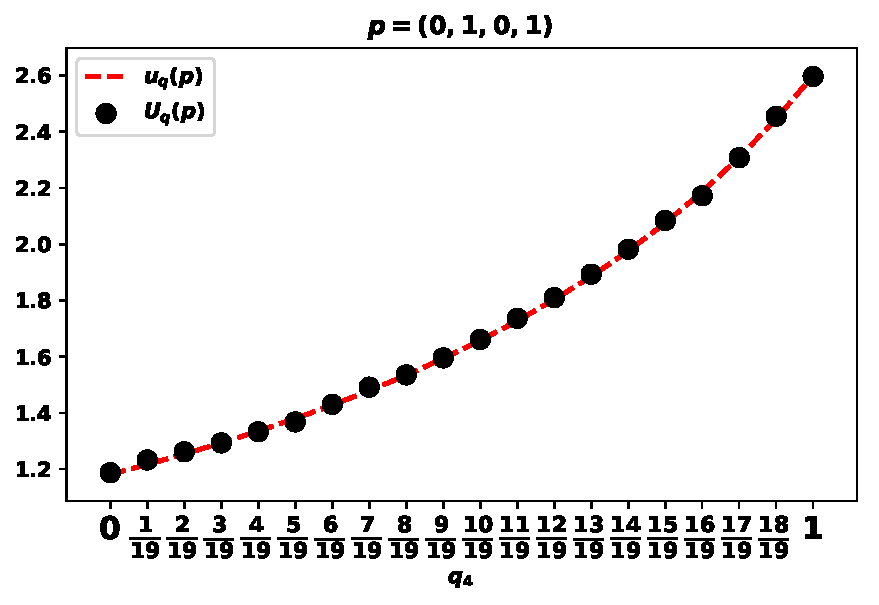
\includegraphics[width=\linewidth]{img/validation_against_player_one.pdf}
        \end{subfigure}
        \begin{subfigure}{0.45\textwidth}
            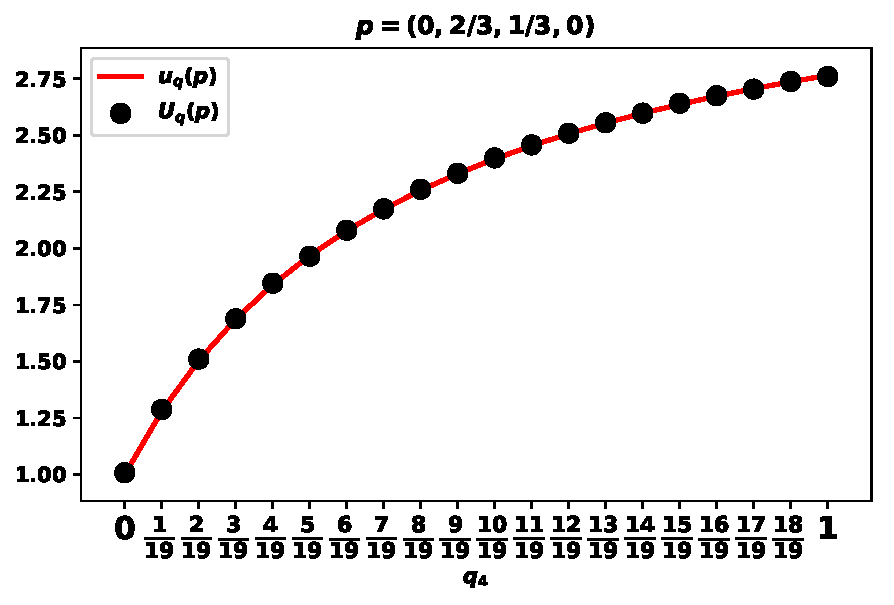
\includegraphics[width=\linewidth]{img/validation_against_player_two.pdf}
        \end{subfigure}
    \end{center}

    \caption{Differences between simulated and analytical results for
            \(q = (\frac{1}{3}, \frac{1}{3}, \frac{1}{3}, q_4)\).}
    \label{fig:analytical_simulated}
\end{figure}

Theorem~\ref{theorem:quadratic_form_u} can be extended to consider multiple
opponents. The IPD is commonly studied in tournaments and/or Moran Processes
where a strategy interacts with a number of opponents. The payoff of a player in
such interactions is given by the average payoff the player received against
each opponent. More specifically the expected utility of a memory one strategy
against a \(N\) number of opponents is given by
Theorem~\ref{theorem:tournament_utility}.

\begin{theorem}\label{theorem:tournament_utility}
    The expected utility of a memory one strategy \(p\in\mathbb{R}_{[0,1]}^4\)
    against a group of opponents \(q^{(1)}, q^{(2)}, \dots, q^{(N)}\), denoted
    as \(\frac{1}{N} \sum\limits_{i=1} ^ {N} {u_q}^{(i)} (p)\) is given by:

    \begin{equation}\label{eq:tournament_utility}
        \frac{1}{N} \sum\limits_{i=1} ^ {N} {u_q}^{(i)} (p) = \frac{1}{N}
        \frac{\sum\limits_{i=1} ^ {N} (\frac{1}{2} pQ^{(i)} p^T + c^{(i)} p + a^ {(i)})
        \prod\limits_{\tiny\begin{array}{l} j=1 \\ j \neq i \end{array}} ^
        N (\frac{1}{2} p\bar{Q}^{(i)} p^T + \bar{c}^{(i)} p + \bar{a}^ {(i)})}
        {\prod\limits_{i=1} ^ N (\frac{1}{2} p\bar{Q}^{(i)} p^T + \bar{c}^{(i)} p + \bar{a}^ {(i)})}.
    \end{equation}
\end{theorem}

Theorem~\ref{theorem:tournament_utility} is validated against the strategies
used in~\cite{Stewart2012}, Figure~\ref{fig:stewart_plotkin_results}.
A list of the strategies is given by Table~\ref{table:list_stewart_plotkin}.

\begin{table}
        \begin{center}
        \resizebox{.5\textwidth}{!}{\begin{tabular}{clcc}
        \toprule
        {}&  Name & Memory one representation & Reference \\
        \midrule
        1  & Cooperator           & \((1, 1, 1, 1)\) & \cite{Axelrod1981} \\
        2  & Defector             & \((0, 0, 0, 0)\) & \cite{Axelrod1981}\\
        3  & Random               & \((\frac{1}{2}, \frac{1}{2}, \frac{1}{2},
        \frac{1}{2})\) & \cite{Axelrod1981} \\
        4  & Tit for Tat          & \((1, 0, 1, 0)\) & \cite{Axelrod1981}\\
        5  & Grudger              & \((1, 0, 0, 0)\) & \cite{Li2011} \\
        6  & Generous Tit for Tat & \((1, \frac{1}{3}, 1, \frac{1}{3})\) & \cite{Nowak1990}\\
        7  & Win Stay Lose Shift  & \((1, 0, 0, 1)\) & \cite{Nowak1993} \\
        8  & ZDGTFT2              & \((1, \frac{1}{8}, 1, \frac{1}{4})\) &\cite{Stewart2012}\\
        9  & ZDExtort2            & \((\frac{8}{9}, \frac{1}{2}, \frac{1}{3},
        0)\) & \cite{Stewart2012}\\
        10 & Hard Joss            & \((\frac{9}{10}, 0, \frac{9}{10}, 0)\) &
        \cite{Stewart2012} \\
        \bottomrule
    \end{tabular}}
    \caption{List of strategies used in the tournament described in~\cite{Stewart2012}.}
    \label{table:list_stewart_plotkin}
    \end{center}
\end{table}

\begin{figure}[!htbp]
    \begin{center}
    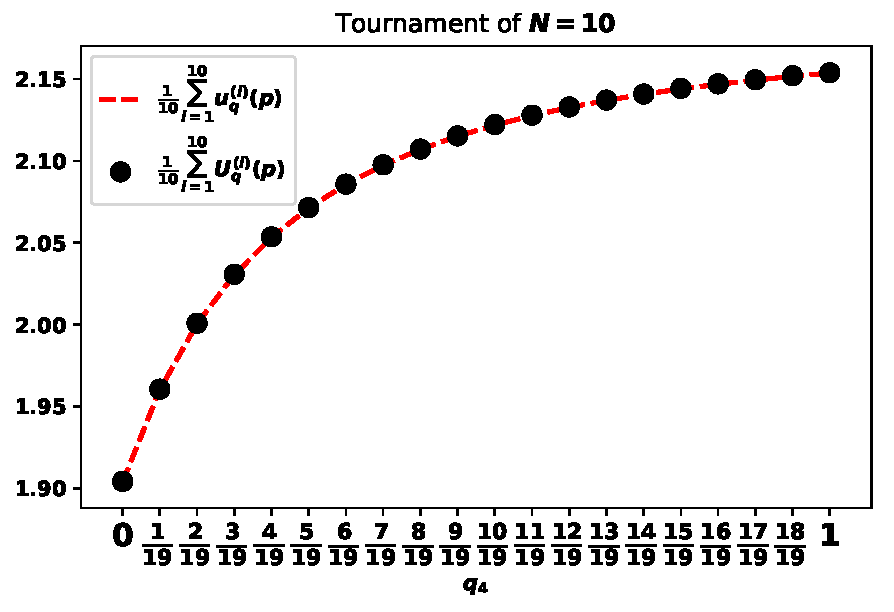
\includegraphics[width=.5\linewidth]{img/Stewart_tournament_results.pdf}
    \caption{Results of memory one strategies against the strategies in
    Table~\ref{table:list_stewart_plotkin}.}
    \label{fig:stewart_plotkin_results}
    \end{center}
\end{figure}

Furthermore, using the same list of strategies the 
hypothesis the utility against a group of strategies could be
captured by the utility against the mean opponent, thus:

\begin{equation}\label{eq:condition}
    \frac{1}{N} \sum_{i=1} ^ {N} {u_q}^{(i)} (p) = u_{\frac {1}{N} \sum\limits_{i=1} ^ N q^{(i)}}(p),
\end{equation}

has been checked. The hypothesis fails and numerical evidence are given by
Figure~\ref{fig:hypothesis}.

\begin{figure}[!htbp]
    \begin{center}
    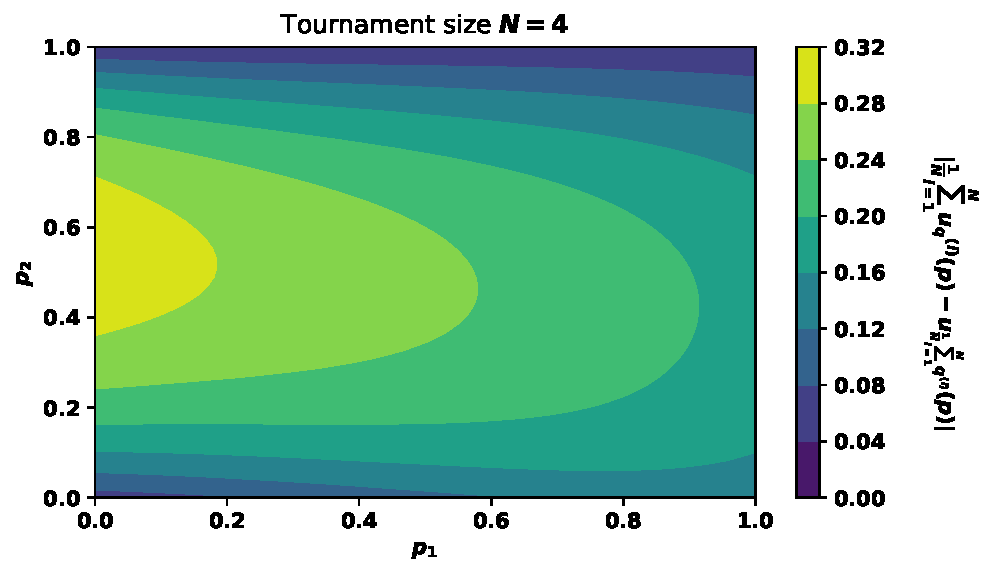
\includegraphics[width=.5\linewidth]{img/mean_vs_average_heatmap.pdf}
    \end{center}
    \caption{The difference between the average utility and against
    the utility against the average player of the strategies in~\cite{Stewart2012}.
    A positive difference indicates that the condition (\ref{eq:condition})
    does not hold.}
    \label{fig:hypothesis}
\end{figure}

Theorem~\ref{theorem:tournament_utility} can be used to identify best
responses in the case of memory one strategies. In the following sections several
theoretical results are presented and the advantages of analytical formulation
of become evident.

\section{Best responses to memory one players}\label{section:best_response_mem_one}

A \textit{best response} is the strategy which corresponds to the most
favourable outcome. A best response memory one strategy
corresponds to the \(p^*\) for which \(\sum u_{q ^{(i)}} (p^*)\) for \(i \in \{1, \dots, N\}\)
is maximized. This is considered as a multi dimensional optimisation problem
where the decision variable is the vector \(p\), the solitary constraint is
that \(p \in \R^4_{[0, 1]} \) and the objective function is a sum of quadratic
ratios. The optimisation problem is formally given by~(\ref{eq:mo_tournament_optimisation}).

\begin{equation}\label{eq:mo_tournament_optimisation}
    \begin{aligned}
    \max_p: & \ \sum_{i=1} ^ {N} {u_q}^{(i)} (p)
    \\
    \text{such that}: & \ p \in \R_{[0, 1]}
    \end{aligned}
\end{equation}

Optimising this particular ratio of quadratic forms is not trivial. It can be
verified empirically for the case of a single opponent that there exist at least
one point for which the definition of concavity does not hold. There is some
work on the optimisation on non concave ratios of quadratic forms
\cite{Beck2009, Hongyan2014}, in these both the numerator and the denominator of
the fractional problem were concave or that the denominator was greater than
zero. Both assumptions fails for (\ref{eq:mo_tournament_optimisation}). These
results are established in Theorem~\ref{theorem:concavity}.

\begin{theorem}\label{theorem:concavity}
    The utility of a player \(p\) against an opponent \(q\), \(u_q (p)\) given by
    (\ref{eq:optimisation_quadratic}), is not concave. Furthermore neither the
    numeration or the denominator of (\ref{eq:optimisation_quadratic}), are concave.
\end{theorem}

The non concavity of \(u(p)\) indicates multiple local optimal points. The
approach taken here is to introduce a compact way of constructing the candidate
set of all local optimal points. Once the set is defined the point that
maximises (\ref{eq:tournament_utility}) corresponds to the best response
strategy, this approach transforms the continuous optimisation problem in to a
discrete problem. The problem considered is a bounded because \(p \in \R^4_{[0,
1]}\). The candidate solutions will exist either at the boundaries of the
feasible solution space, or within that space. The method of Lagrange
Multipliers~\cite{bertsekas2014} and Karush-Kuhn-Tucker
conditions~\cite{Giorgi2016} are based on this. The Karush-Kuhn-Tucker
conditions are used here because the constraints are inequalities.
These lead to Lemma~\ref{lemma:memone_group_best_response} which
presents the best response memory one strategy to a group of opponents.

\begin{lemma}\label{lemma:memone_group_best_response}

    The optimal behaviour of a memory one strategy player
    \(p^* \in \R_{[0, 1]} ^ 4\)
    against a set of \(N\) opponents \(\{q^{(1)}, q^{(2)}, \dots, q^{(N)} \}\)
    for \(q^{(i)} \in \R_{[0, 1]} ^ 4\) is established by:

    \[p^* = \textnormal{argmax}(\sum\limits_{i=1} ^ N  u_q(p)), \ p \in S_q.\]

    The set \(S_q\) is defined as all the possible combinations of:

    \begin{itemize}
    \item Any one, two, three, four or non of the transition probabilities of
    \(p\) are zero,
    \item while any one, two, three, four or non of the transition probabilities of
    \(p\) are one,
    \item while any one, two, three, four or non of the transition probabilities of
    \(p\) are the roots of \(\frac{d}{dp} \sum\limits_{i=1} ^ N  u_q(p)\).
    \end{itemize}

\end{lemma}

Equation (\ref{eq:derivative_numerator_condition}) is systems of at most \(4\)
polynomials and the degree of the polynomials is gradually increasing every time
an extra opponent is taken into account.
%TODO add sentence and (see Appendix) on how this is solved for a constrainted
% version of the reactive case. Briefly comment on resultants. Though severals
% for larger system does exist
Solving system of polynomials corresponds to the calculation of a resultant and
for large systems these quickly become intractable.
% TODO Add a reference here about resultants.
Because of that no further analytical consideration is given to problems
described here

\section{Stability of defection}

Defection is known to be the dominant action in the PD and it can be proven to
be the dominant strategy for the IPD for given environments. Even so, several
works have proven that cooperation emerges in the IPD and many studies focus on
the emergence of cooperation. This manuscript provides an identification of
conditions for which defection is known to be a best response; thus identifying
environments where cooperation can not occur, Lemma~\ref{lemma:stability_of_defection}.

\begin{lemma}\label{lemma:stability_of_defection}
    In a tournament of \(N\) players where \(q^{(i)} = (q_{1}^{(i)}, q_{2}^{(i)}, q_{3}^{(i)}, q_{4}^{(i)})\)
    defection is a best response if the transition probabilities of the
    opponents satisfy the condition:

    \begin{equation}
        \sum_{i=1} ^ N (c^{(i)T} \bar{a}^{(i)} - \bar{c}^{(i)T} a^{(i)}) \leq 0
    \end{equation}
\end{lemma}

\begin{proof}
    For defection to be evolutionary stable the derivative of the utility
    at the point \(p = (0, 0, 0, 0)\) must be negative. This would indicate that
    the utility function is only declining from that point onwards.

    Substituting \(p = (0, 0, 0, 0)\) in
    equation~(\ref{eq:mo_tournament_derivative}) which gives:

    \begin{equation}
    \sum_{i=1} ^ N (c^{(i)T} \bar{a}^{(i)} - \bar{c}^{(i)T} a^{(i)})
    \prod\limits_{\tiny\begin{array}{l} j=1 \\ j \neq i \end{array}} ^ N (\bar{a}^{(i)})^2
    \end{equation}
    
    The second term \(\prod\limits_{\tiny\begin{array}{l} j=1 \\ j \neq i
    \end{array}} ^ N (\bar{a}^{(i)})^2\) is always positive,however, the sign of the
    first term \(\sum_{i=1} ^ N (c^{(i)T} \bar{a}^{(i)} - \bar{c}^{(i)T} a^{(i)})\)
    can vary based on the transition probabilities of the opponents. Thus the
    sign of the derivative is negative if and only if
    \(\sum_{i=1} ^ N (c^{(i)T} \bar{a}^{(i)} - \bar{c}^{(i)T} a^{(i)}) \leq 0\).
\end{proof}


\section{Numerical experiments and Results} \label{section:numerical_experiments}

In this section best responses are explored numerically. Best responses are
estimated using the Bayesian optimisation algorithm. Bayesian optimisation is a
global optimisation algorithm, introduced in~\cite{Mokus1978}, which has proven
to outperform many other popular algorithms~\cite{Jones2001}. Differential
evolution had also been considered, however it was not chosen due to Bayesian
being computationally faster.

The algorithm can be used to solve the problem of
(\ref{eq:mo_tournament_optimisation}). Consider an example
where \(N=2\), for a given number of calls the algorithm tries to find \(p^*\)
such that the utility is maximized. Figure~\ref{bayesian_example} illustrates
the change of the utility function over number of calls.

The default number of iterations that have been used in this work is 60. After
the 60 calls the convergence of the utility is checked. If it is not then the
calls are increased by 20, this step is then repeated until the utility reaches
convergence.

\begin{figure}[!htbp]
    \begin{center}
    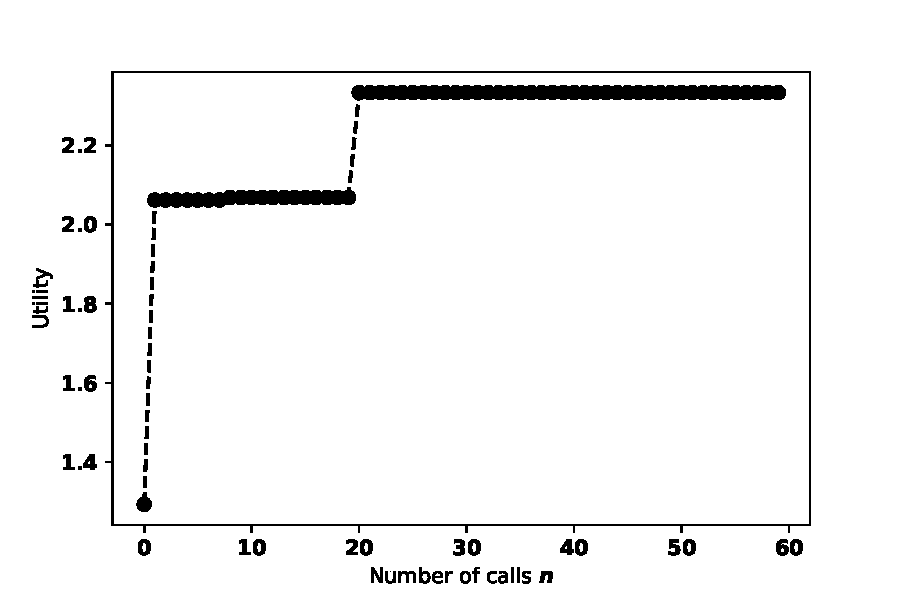
\includegraphics[width=.5\linewidth]{img/bayesian_example.pdf}
    \end{center}
    \caption{Utility over time of calls using Bayesian optimisation. The
    opponents are \(q^{(1)} = (\frac{1}{3}, \frac{1}{3}, \frac{1}{3},
    \frac{1}{3})\) and \(q^{(2)} = (\frac{1}{3}, \frac{1}{3},
    \frac{1}{3}, \frac{1}{3})\).}
    \label{bayesian_example}
\end{figure}

A series of experiments are carried out and Bayesian optimisation is used to
estimate the best responses for different settings. Such as:

\begin{itemize}
    \item Memory one best responses to \(N=2\) opponents.
    \item Memory one best responses in evolutionary dynamics.
    \item Longer memory best responses.
\end{itemize}

The details of the experiments and their results are presented in the following
subsections.

\subsection{Memory one best responses for \(N=2\)}\label{subsection:best_response_n_2}

The first experiment that has been carried out is estimating the memory one
best responses in a tournament with two opponents. \(N=2\) has been chosen as it's
the smallest size of a tournament. For each trial of the experiment a set of
2 opponents is randomly generated, the memory one best response against them
is calculated and it's behaviour is being recorded. A total of 1000 trials have
been recorded. The data have archived and found at.

Though the probabilities \(q_i\) of the opponents are randomly generated,
Figure~\ref{fig:opponents_probabilities} shows that they are uniformly distributed.
Thus, the space full space of possible opponents has been covered.

\begin{figure}[!htbp]
    \begin{subfigure}{0.49\textwidth}
        \centering
        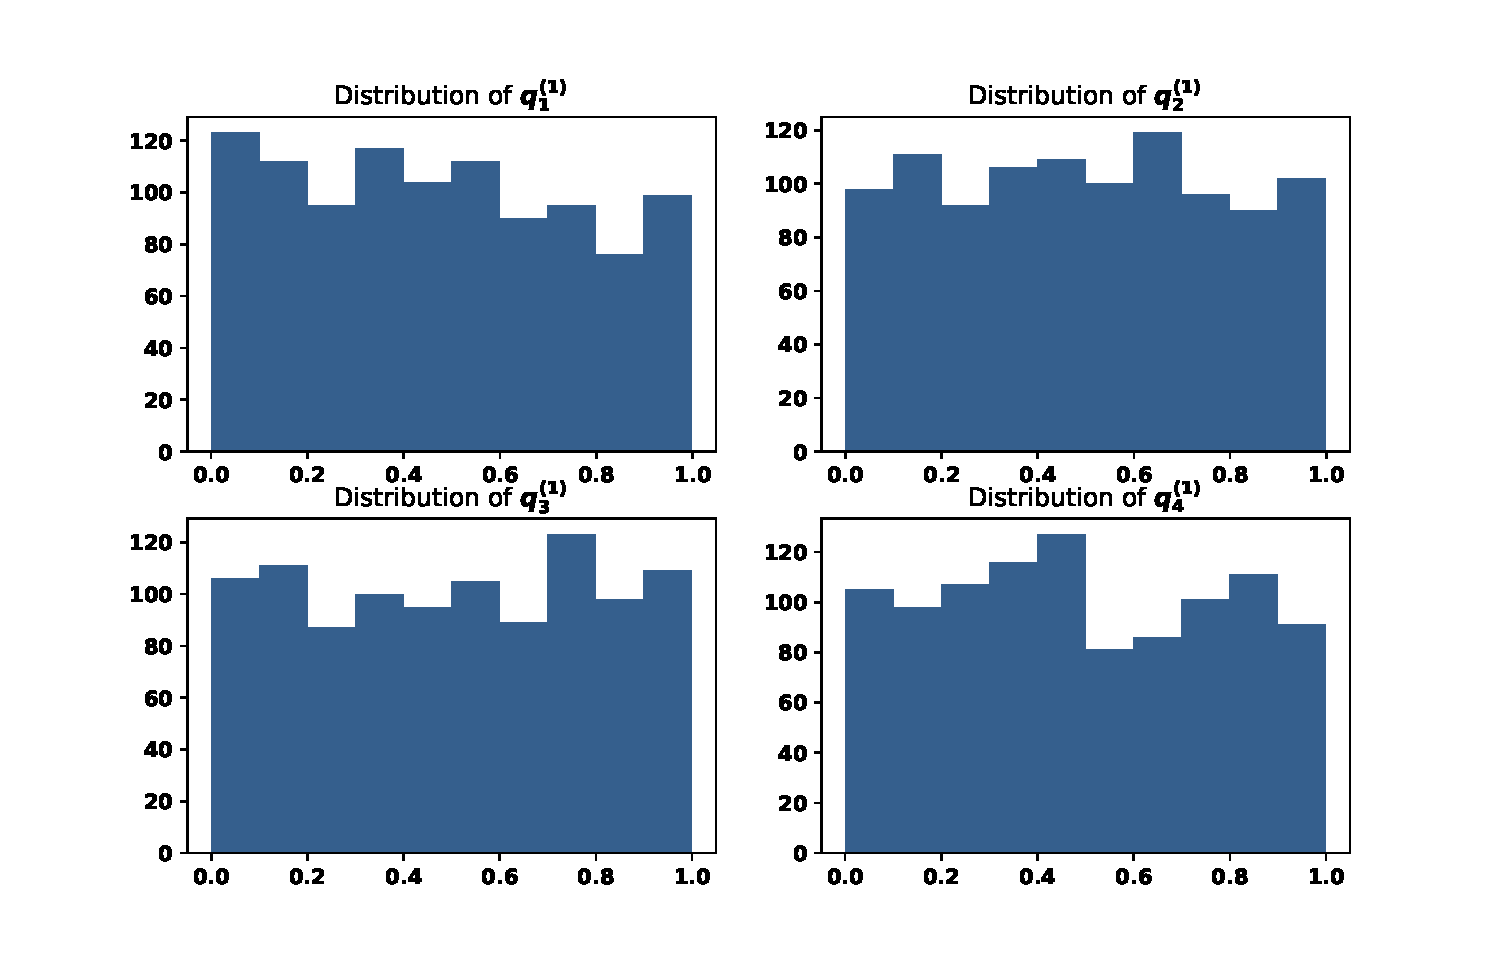
\includegraphics[width=\linewidth]{img/first_opponent_probabilities.pdf}
        \subcaption{Distributions of opponents' probabilities.}
        \label{fig:opponents_probabilities}
    \end{subfigure}
    \begin{subfigure}{0.49\textwidth}
        \centering
        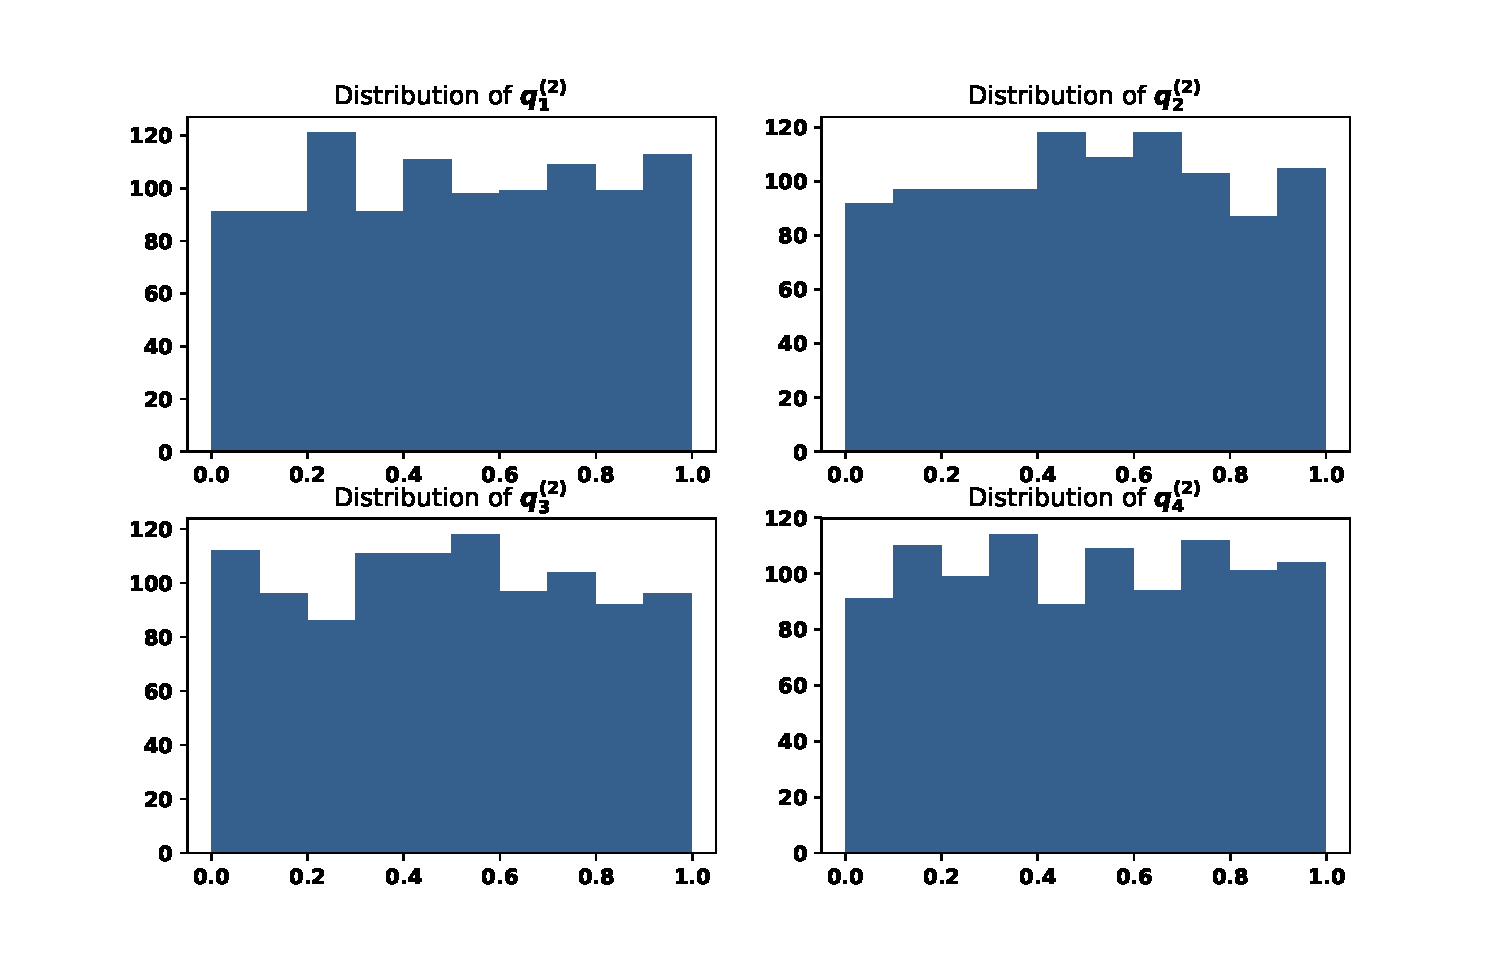
\includegraphics[width=\linewidth]{img/second_opponent_probabilities.pdf}
        \subcaption{Distributions of opponents' probabilities.}
        \label{fig:opponents_probabilities}
    \end{subfigure}
\end{figure}

Section~\ref{section:introduction} discussed ZD strategies and their robustness
against a single opponent. ZD strategies control their opponent's score and thus
are able to always receive a higher payoff than them. In tournament settings,
where more than 2 strategies interact, winning at each single interaction does
not guaranty a strategy's overall win. This manuscript argues that ZD do not
receive the most favoured payoff from their interactions and thus come sort in a
tournament setting environment.

Best responses are strategies that aim to gain the most of their entire opponent
set. In [Knight 2019] a method of measuring the extortionate behaviour of a
strategy, based on it's estimated probabilities, has been defined. The method
allows to estimate the error of behaving as a ZD strategy, SSerror. The SSerror
method is applied on the data set of this work. The distribution of the error is
shown in Figure~\ref{fig:sserror_mem_one} and a statistics summary by
Table~\ref{table:sserror_stats} (outliers have been removed).

The mean and median of the SSerror are estimated at 1.5. With a tolerance of 0.1,
only 25 percent of the memory one best responses appear to be behaving in an
extortionate way. Moreover, a positive measure of skewness \((=0.94)\), indicates
that the distribution is skewed to the right. 

\begin{figure}
    \begin{minipage}{0.59\textwidth}
            \begin{center}
            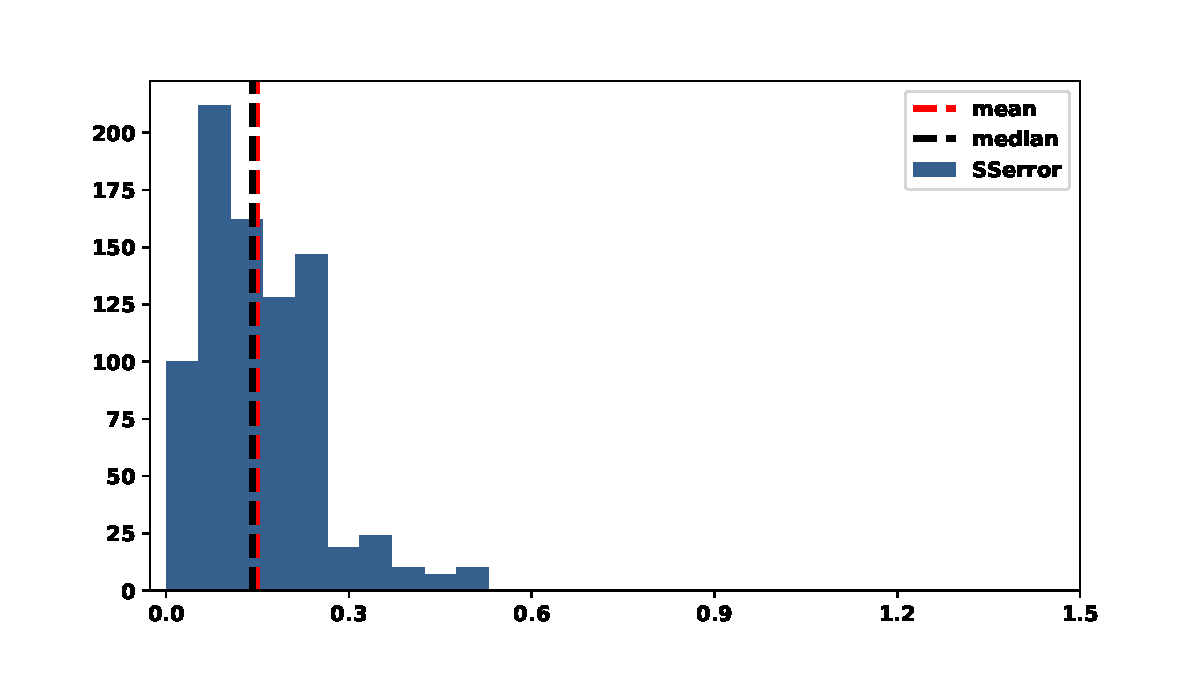
\includegraphics[width=\linewidth]{img/best_respones_sserror_remove_outliers.pdf}
            \end{center}
            \caption{Distribution of sserrors for memory one best responses, when \(N=2\).}
            \label{fig:sserror_mem_one}
    \end{minipage}
    \hfill
    \begin{minipage}{0.39\textwidth}
        \centering
        \captionsetup{type=table}
        \resizebox{.4\columnwidth}{!}{%
            \begin{tabular}{lr}
\toprule
{} &     SSerror \\
\midrule
count &  819.000000 \\
mean  &    0.148246 \\
std   &    0.100002 \\
min   &    0.000000 \\
25\%   &    0.058824 \\
30\%   &    0.066779 \\
35\%   &    0.093944 \\
50\%   &    0.142050 \\
max   &    0.529412 \\
\bottomrule
\end{tabular}
}
            \caption{Summary statistics SSerror}
            \label{table:sserror_stats}
      \end{minipage}
\end{figure}

Overall only a very small percentage of the best responses seem to behaving in
an extortionate way, confirming our original hypothesis. That ZD strategies do
not gain the maximum outcome from their interactions. The following section the
second experiment and the result of memory one best responses in evolutionary
dynamics are presented.

\subsection{Memory one best responses in evolutionary dynamics}

As briefly discussed in Section~\ref{section:utility}, the IPD is commonly
studied in Moran Processes, and generally in evolutionary processes. In
evolutionary processes, a finite population is assumed where the strategies that
compose the population can adapt and change their behaviour based on the
outcomes of their interactions at each turn. A key in successfully being an
evolution stable strategy (ESS) is self interactions. An ESS must be a best
response not only to the opponents in the population, but also it has to be a
best response to it's self.

Self interactions can easily be incorporated in the formulation that has been used
in this paper. The utility of a memory one strategy in an evolutionary setting
is given by,

\begin{equation}
    \frac{1}{N} \sum\limits_{i=1} ^ {N} {u_q}^{(i)} (p) + u_p(p).
\end{equation}

and respectively the optimisation problem of (\ref{eq:mo_tournament_optimisation})
is now re written as,

\begin{equation}\label{eq:mo_evolutionary_optimisation}
    \begin{aligned}
    \max_p: & \ \frac{1}{N} \sum\limits_{i=1} ^ {N} {u_q}^{(i)} (p) + u_p(p)
    \\
    \text{such that}: & \ p \in \R_{[0, 1]}
    \end{aligned}
\end{equation}

Due to the new term being added to the utility, the assumption that has been
made so far regarding the form of the utility now fails. The utility is not
a ratio of two quadratic forms any more. Furthermore, a new method for
identifying an evolutionary best response is composed in this Section.
The method considered is called \textit{best response dynamics}, and the algorithm
describing the method is given by Algorithm~\ref{algo:best_response_dynamics}.

Best response dynamics are commonly used in evolutionary game theory. Best
response dynamics represent a class of strategy updating rules, where players
strategies in the next round are determined by their best responses to some
subset of the population, whether this might be in a large population model
such as Moran Processes~\cite{Knight2018} or in a spatial model~\cite{Nowak1992}.
Moreover, in the theory of potential games, best response dynamics
refers to a way of finding a pure Nash equilibrium by computing the best response for
every player~\cite{Nisan2007}. Here we defined a combination of the two methods.

%\begin{algorithm}
    \setstretch{1.35}
    \caption{Best response dynamics algorithm}\label{algo:best_response_dynamics}
    \begin{algorithmic}[1]
    \Procedure{Approximate best evolutionary response}{}
    \State $\tilde{p} \gets (0, 0, 0, 0)$
    \State $p^* \gets (1, 1, 1, 1)$
    \While{$p^* \neq \tilde{p}$}:
    \State \text{temp} $\gets \tilde{p}$
    \State $\tilde{p} \gets p^*$
    \State $p^* = \text{argmax}_{p^*}(\sum\limits_{i=1} ^ N  u_q(p^*)) + u_{\text{temp}}(p^*))$ 
    \EndWhile
    \State \textbf{return} $p^*$;
    \EndProcedure
    \end{algorithmic}
\end{algorithm}


\begin{algorithm}[H]
    $p^{(t)}\leftarrow (1, 1, 1, 1)$\;
    \While{$p^{(t)}$ not converged}{
     $p^{(t + 1)} =  \text{argmax} \frac{1}{N} \sum\limits_{i=1} ^ {N} {u_q}^{(i)} (p + 1) + u_p(p + 1)$\;
    }
    \caption{Best response dynamics Algorithm}
\end{algorithm}

Numerical simulations have been carried out to visualise how the algorithm
convergences after a few iterations. In Figure~\ref{fig:best_response_dynamics_results},
the results are illustrated. The algorithm have been set to start from the point
\((1, 1, 1, 1)\). A more optimal point could be considered, but it has been
shown that the algorithm converges to same optimal solution for different
initial starts. Moreover, in Figure~\ref{fig:best_response_dynamics_results}
it is shown that the algorithm stops once the shame point has been evaluated.

\begin{figure}
    \centering
    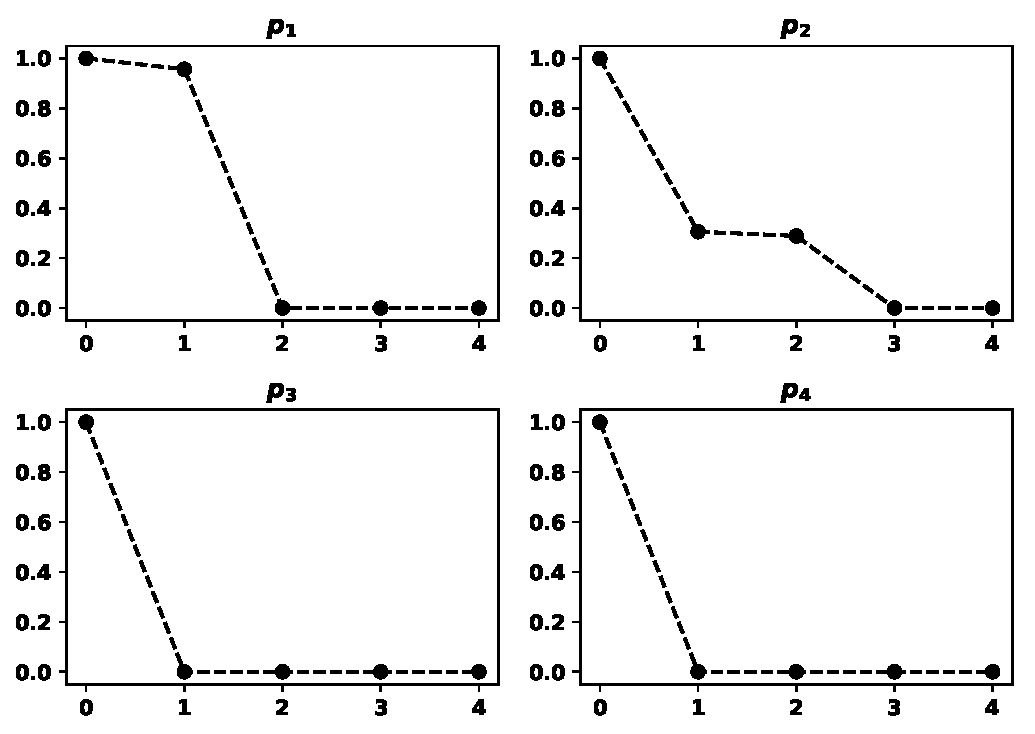
\includegraphics[width=.6\textwidth]{img/evolution_example_two.pdf}
    \caption{Best response dynamics with \(N=2\). More specifically, for
    \(q ^{(1)}=(0.2360,
                0.1031,
                0.3960,
                0.1549)\) and
    \(q ^{(2)}=(0.0665,
                0.4015,
                0.9179,
                0.8004)\).}
\label{fig:best_response_dynamics_results}
\end{figure}

Using the same opponents space as described in Section~\ref{subsection:best_response_n_2},
memory one best evolutionary responses have also been estimated for each trial.
The SSerror for the EVOs is shown in figure~\ref{fig:sserror_mem_one} and
a statistical summary is given by Table~\ref{table:sserror_stats} (outliers have been
removed).

The mean and median of the EVO SSerror are estimated at 1.5, same to the memory
one best responses. It's confirm using a t\-test that there is no significant
difference between the means (p-value \(=0\)). A higher value of skewness
indicates a slightly bigger shift to the right.

\begin{figure}
    \begin{minipage}{0.59\textwidth}
            \begin{center}
            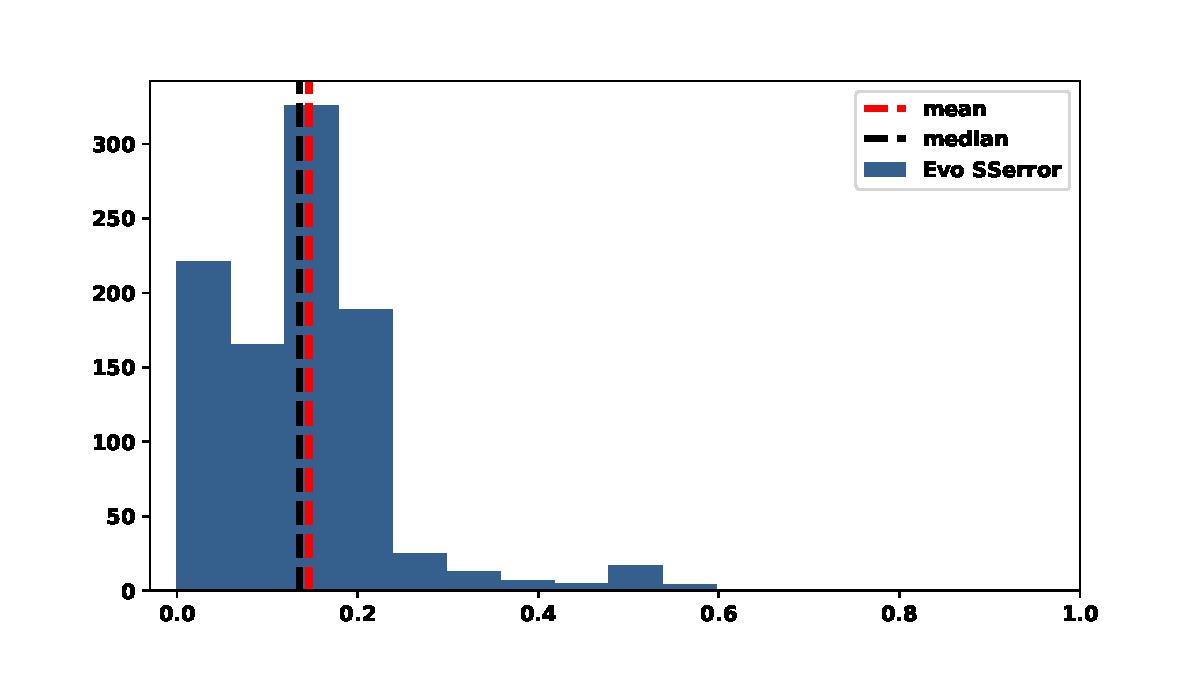
\includegraphics[width=\linewidth]{img/evo_sserror_remove_outliers.pdf}
            \end{center}
            \caption{Distribution of sserrors for memory one best responses, when \(N=2\)}
            \label{fig:sserror_mem_one}
    \end{minipage}
    \hfill
    \begin{minipage}{0.39\textwidth}
        \centering
        \captionsetup{type=table}
        \resizebox{.41\columnwidth}{!}{%
            \begin{tabular}{lr}
\toprule
{} &  Evo SSerror \\
\midrule
count &   972.000000 \\
mean  &     0.146091 \\
std   &     0.097928 \\
min   &     0.000000 \\
25\%   &     0.069945 \\
35\%   &     0.107359 \\
50\%   &     0.135578 \\
75\%   &     0.188117 \\
85\%   &     0.235294 \\
max   &     0.597936 \\
\bottomrule
\end{tabular}
}
            \caption{Summary statistics SSerror}
            \label{table:sserror_stats}
      \end{minipage}
\end{figure}

Similarly to the previous results EVOs do not appear to behave in an extortionate
way. An overview of the difference in behaviour of best responses and EVOs
can be studied by examining the vector probabilities. In Figure~\ref{} the
distributions of each of the cooperating probabilities after each of the four
states is given. The plot has also been evaluated for the 95\% percentile
of the distributions.

\begin{figure}
    \centering
    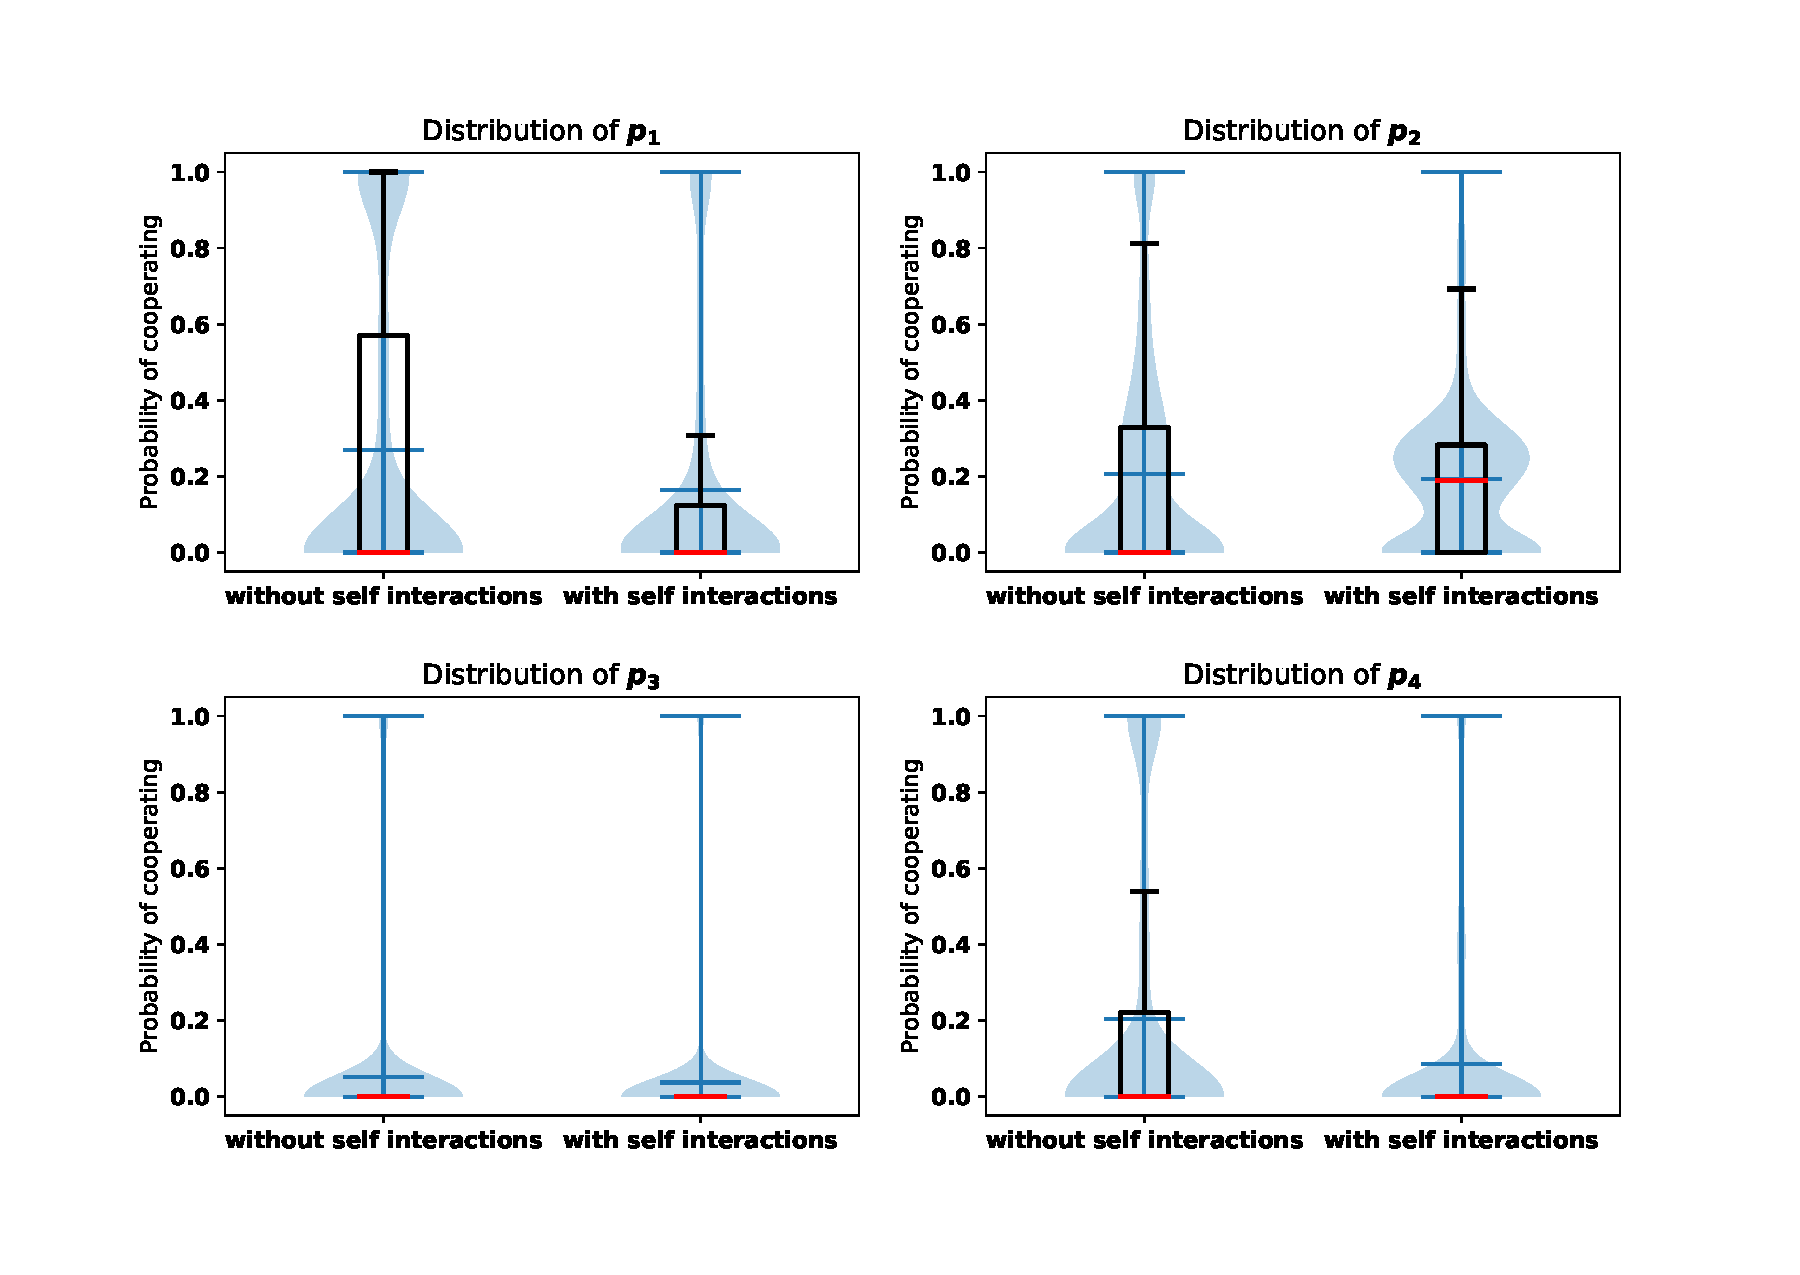
\includegraphics[width=\textwidth]{img/behaviour_violin_plots.pdf}
\end{figure}

\begin{table}
    \begin{tabular}{lrrr}
\toprule
{} &  Memory one Median &  Evo Median &  p-values \\
\midrule
Distribution $p_1$ &                0.0 &    0.000000 &       0.0 \\
Distribution $p_2$ &                0.0 &    0.174359 &       0.0 \\
Distribution $p_3$ &                0.0 &    0.000000 &       0.0 \\
Distribution $p_4$ &                0.0 &    0.000000 &       0.0 \\
\bottomrule
\end{tabular}

\end{table}

\begin{table}
    \begin{tabular}{lr}
\toprule
{} &  Distance Skewness \\
\midrule
\$p\_1\$ difference &           0.220546 \\
\$p\_2\$ difference &          -0.105648 \\
\$p\_3\$ difference &          -7.001084 \\
\$p\_4\$ difference &          -1.937356 \\
\bottomrule
\end{tabular}

\end{table}


\begin{figure}
    \centering
    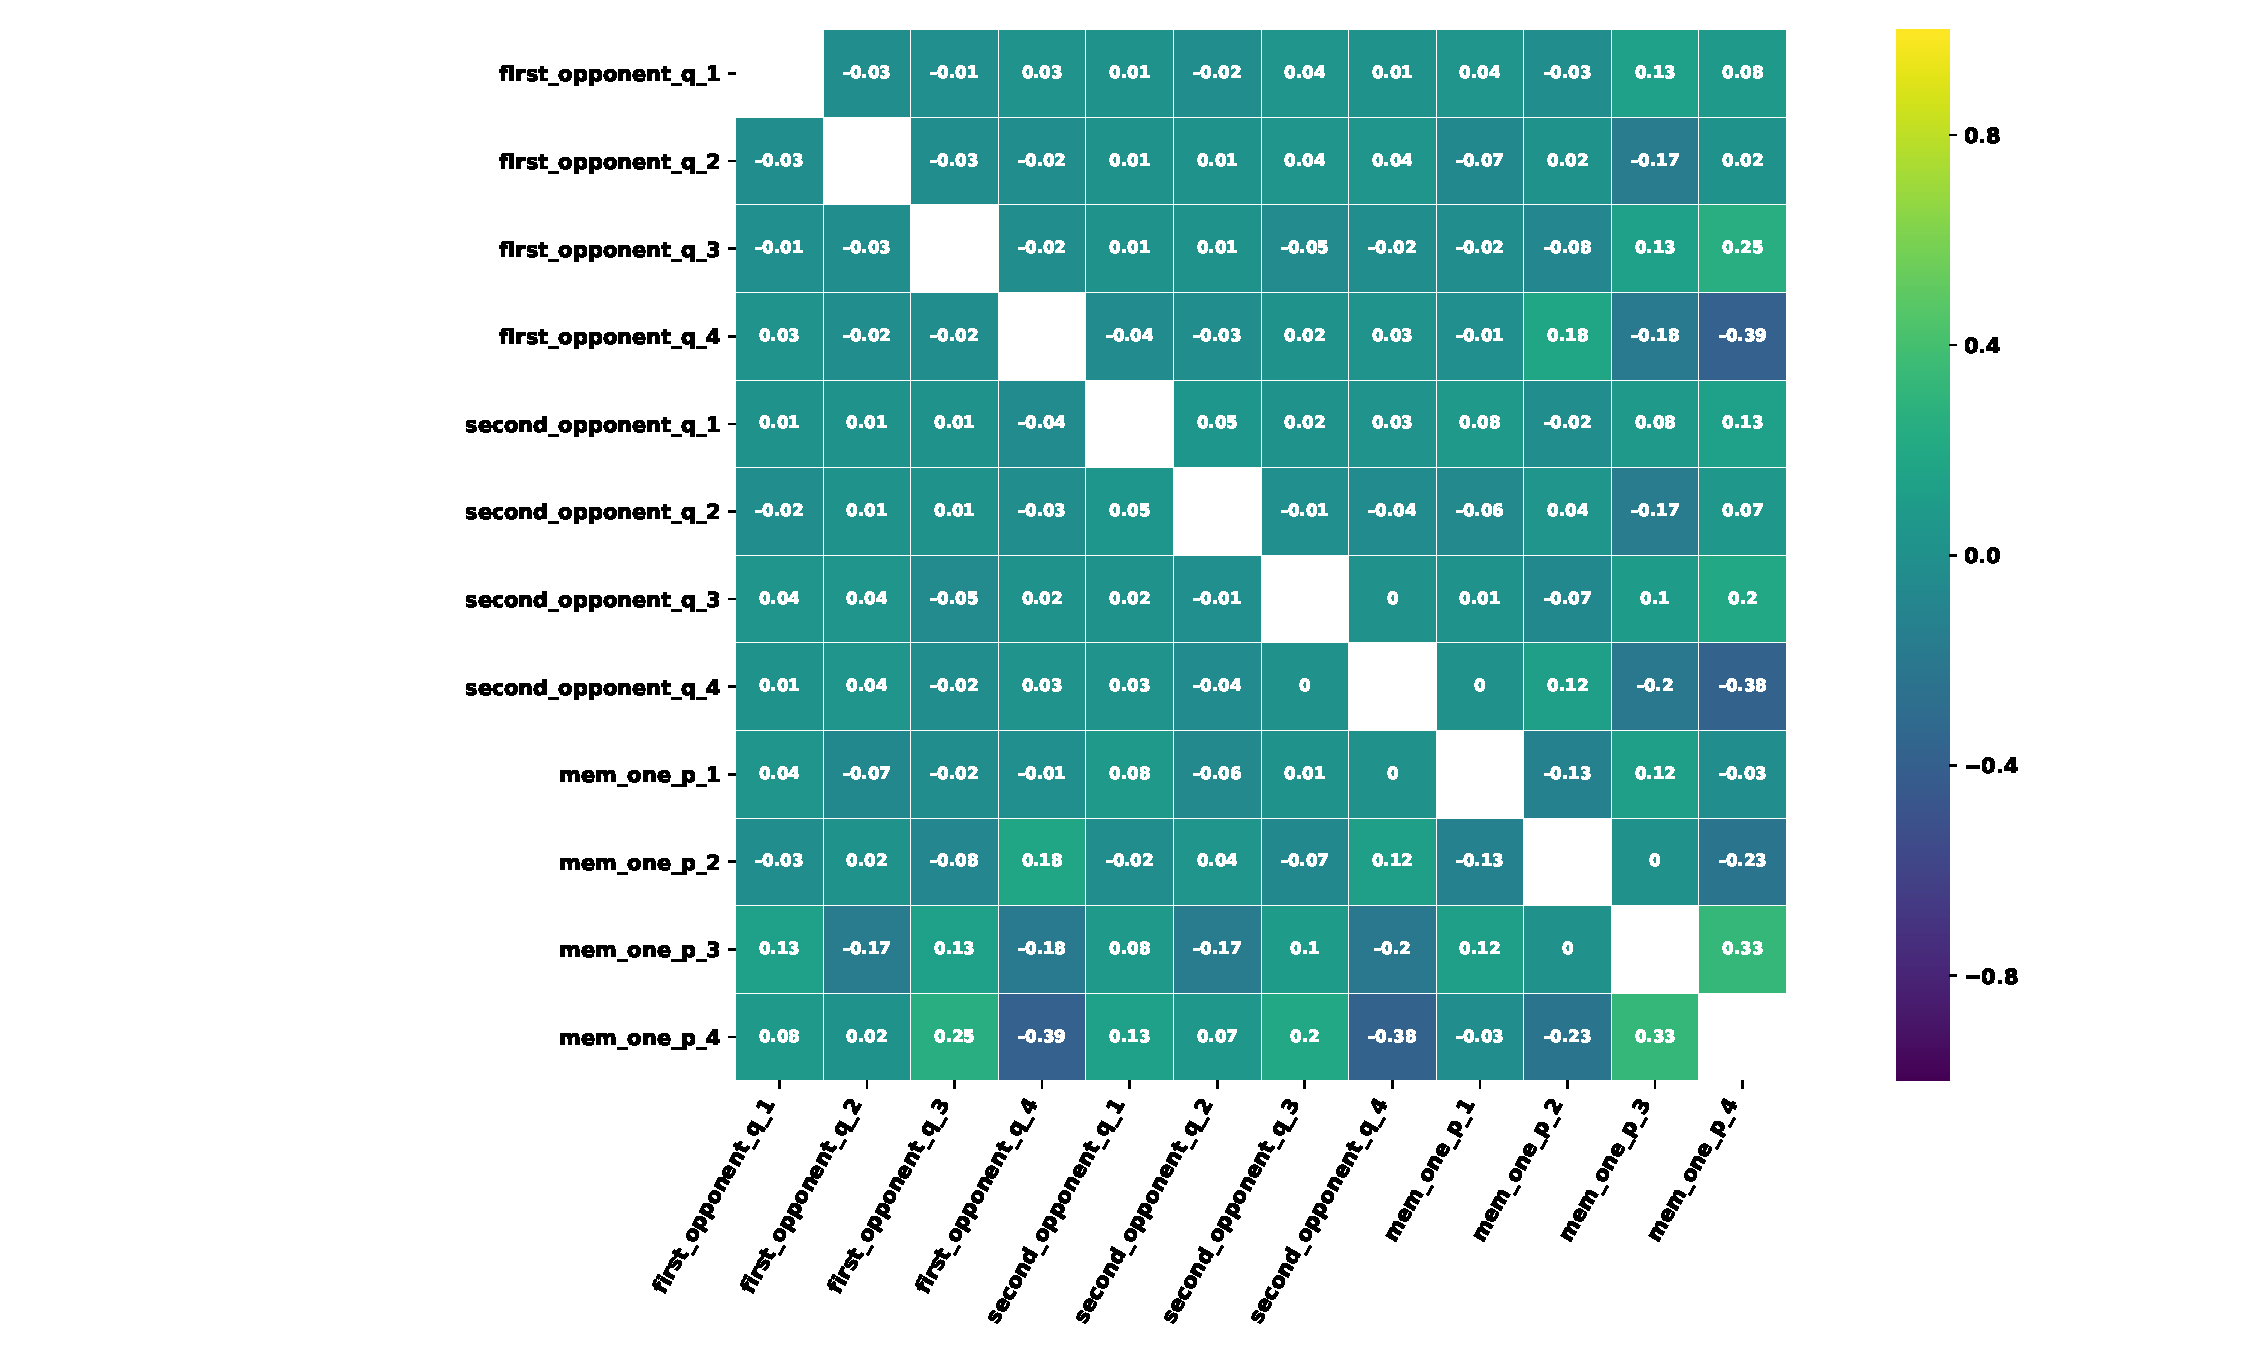
\includegraphics[width=\textwidth]{img/best_response_correlation.pdf}
\end{figure}

\begin{figure}
    \centering
    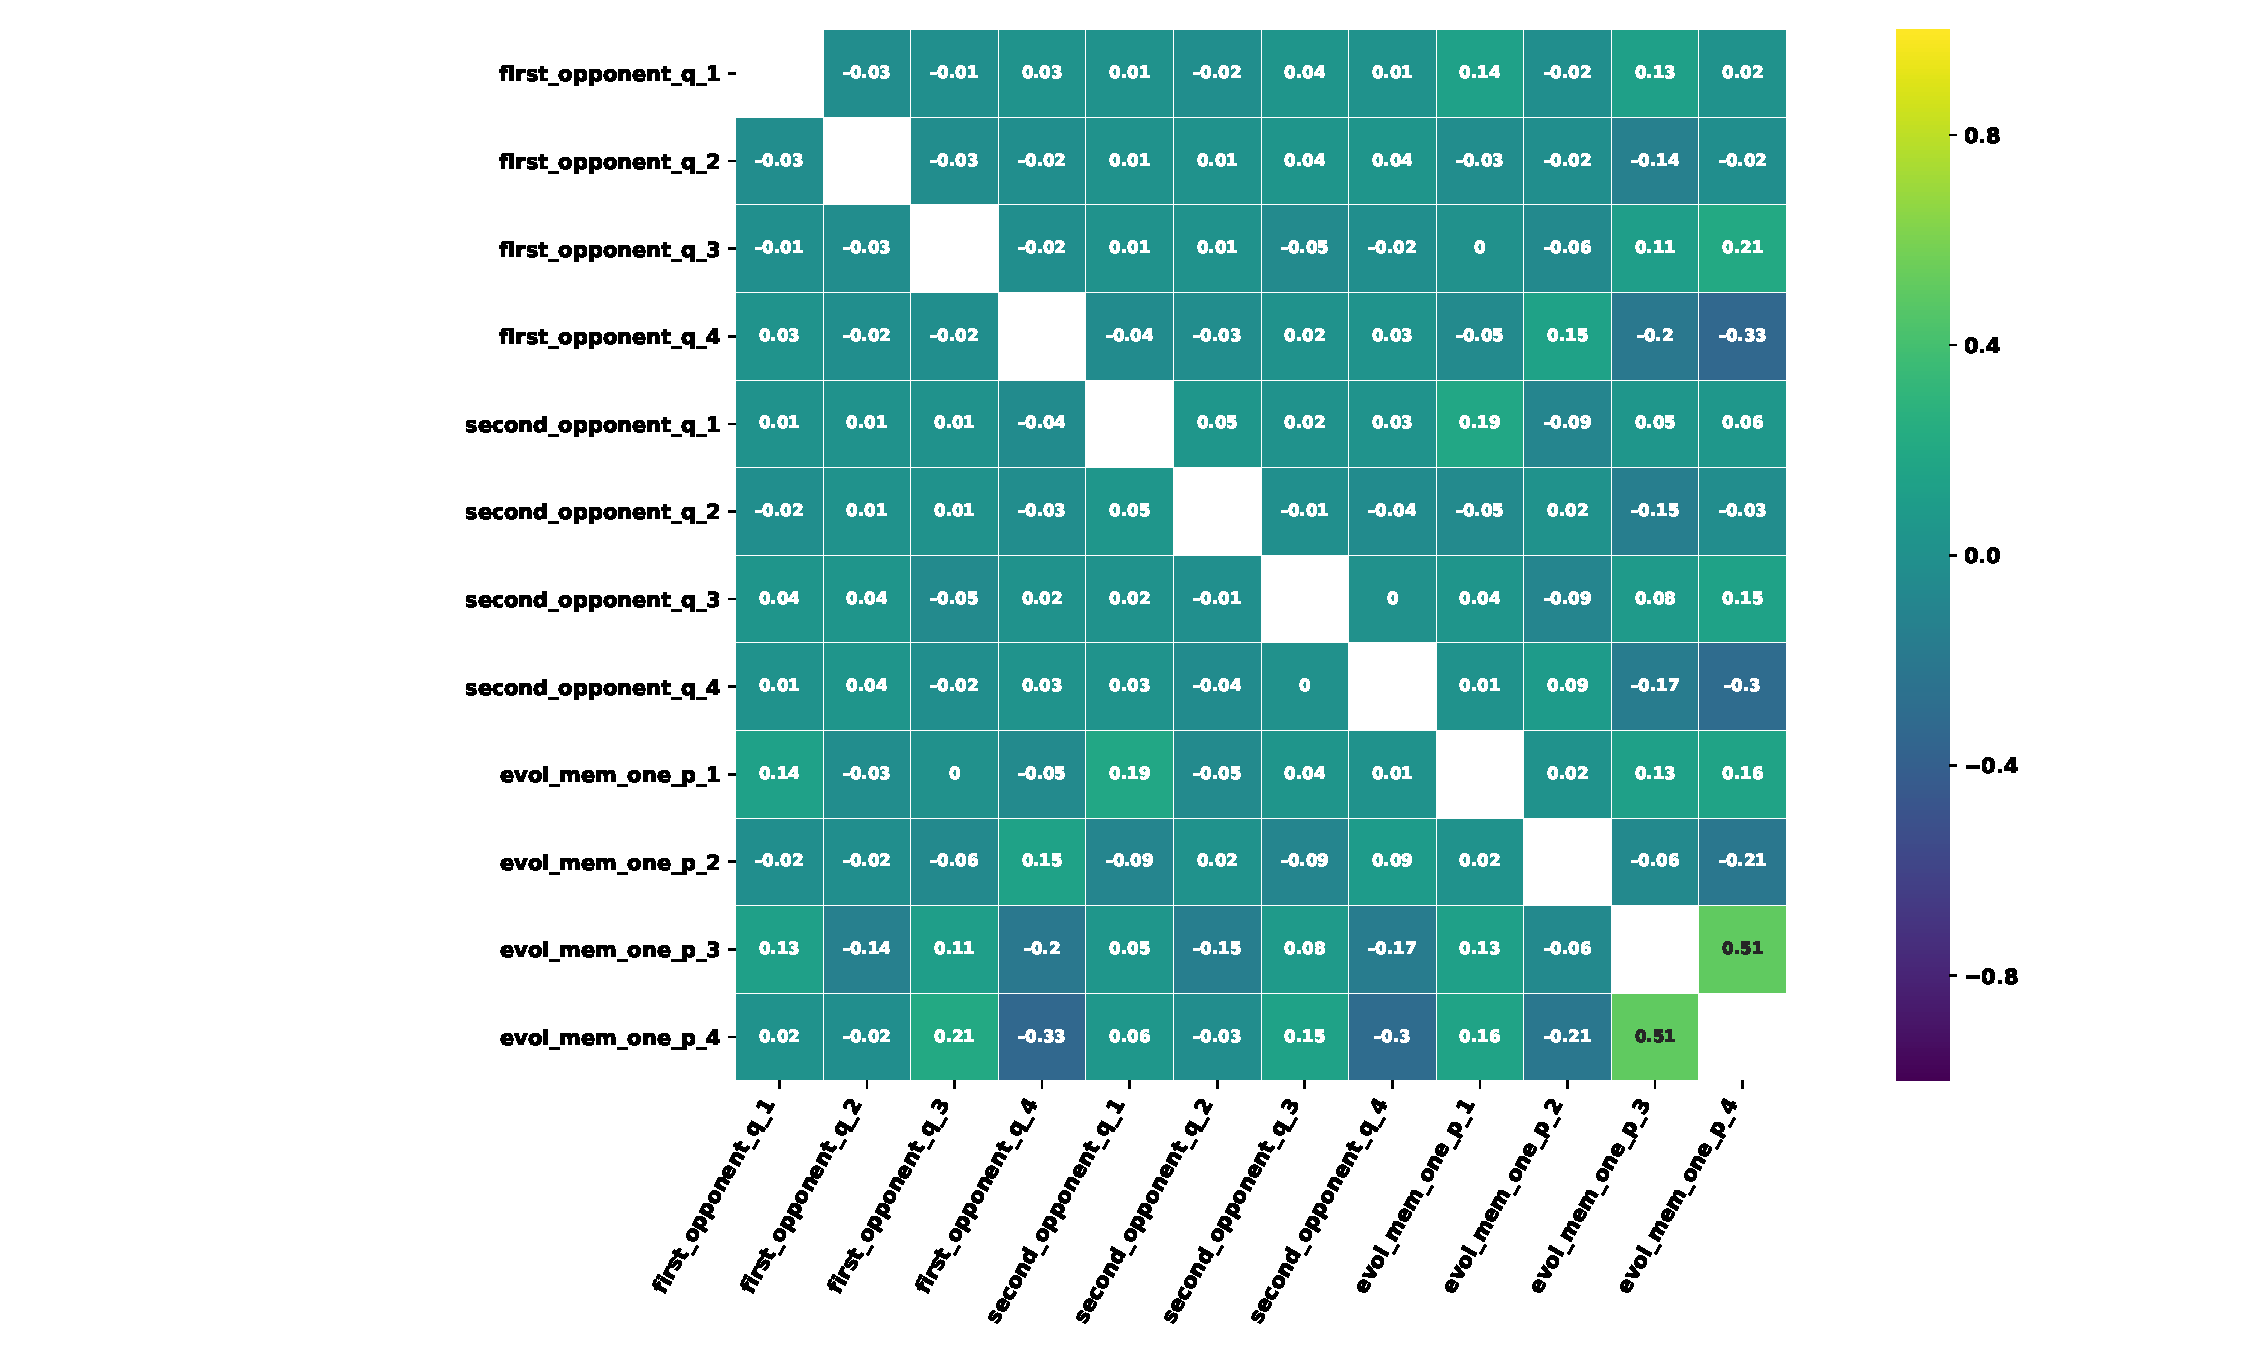
\includegraphics[width=\textwidth]{img/evo_correlation.pdf}
\end{figure}

The difference betwee the 

\section{Longer memory best response}

% The third and final part of this paper focuses on proving that short memory strategies
% have limitations. Though it has been proven~\cite{Press2012} that there exists a set
% of memory one strategies that can outperform any opponent, this was done only for
% the case of \(N=1\). In this section we introduce several empirical results that
% show that more complex strategies can indeed perform better in cases of \(N=2\).
% This is achieved by comparing the performance of an optimised memory one strategy
% to that of a trained long memory one.

% The long memory strategies are trained using reinforcement learning through
% Bayesian optimisation similarly to Section~\ref{section:optimisation_memone}.
% The trained strategy used is a strategy called Gambler,
% introduced and discussed in~\cite{Harper2017}, and the objective function
% is the average performance in a tournament of 200 turns and 50 repetitions.
% Thus, the player learns by playing a number of players, building a Bayesian
% landscape of it's parameters and updating them accordingly.

% \subsection{Gambler}

% Several ways of representing IPD strategies have been used over the years.
% In~\cite{Harper2017} several of those `archetypes' are presented
% and used to train different successful strategies. One of the archetypes firstly
% introduced in that paper is Gambler. Gambler is based on a lookup table and maps
% the opponent's first \(n_1\) moves, the opponent's
% last \(m_1\) moves, and the players last \(m_2\) moves to a probability of
% cooperation.

% Several variants of Gambler have been trained for this work
% (Table~\ref{table:gambler}).

% \begin{table}[htbp]
%     \begin{center}
%     \begin{tabular}{clllll}
%         \toprule
%         {}&  \(n_1\) & \(m_1\) & \(m_2\)\\
%         \midrule
%         1 & 1 & 1 & 2\\
%         2 & 2 & 2 & 0\\
%         3 & 2 & 2 & 1\\
%         4 & 2 & 2 & 2\\
%         5 & 4 & 4 & 4\\
%         \bottomrule
%     \end{tabular}
%     \end{center}
%     \caption{Variants of Gambler used.}
%     \label{table:gambler}
% \end{table}

% \subsection{Empirical Results}

% The performance of the memory one and Gamblers strategies are compared for cases of
% \(N=1\) and \(N=2\). The following steps are taken:

% \begin{enumerate}
%     \item An \(N\) number of random opponents are generated: this gives the
%         environment.
%     \item Using (\ref{eq:mo_tournament_optimisation}) and Bayesian optimisation \(p^*\) 
% s obtained for the environment.
%     \item A Gambler type (each variant of Table~\ref{table:gambler}) is trained for the same environment.
%     \item Both utilities are compared.
% \end{enumerate}

% A large data set containing the opponents as well as the optimised/trained behaviours
% can be found in. %TODO archive
% The number of experimental cases for each Gambler are displayed in Table~\ref{table:number_of_trials_per_gambler}.
% Note that a number of 1022 trials corresponds to 1022 trials for \(N=1\) and 1022
% trials for \(N=2\).

% \begin{table}[htbp]
%     \begin{center}
%     \input{tex/gambler_number_of_trials.txt}
%     \caption{Number of trials, for \(N=1\) and \(N=2\), for each Gambler instance.}
%     \label{table:number_of_trials_per_gambler}
%     \end{center}
% \end{table}

% The results are explored by studying the difference between
% \(\frac{1}{N} \sum\limits_{i=1} ^ {N} {u_q}^{(i)} (p ^ *)\) and
% \(\frac{1}{N} \sum\limits_{i=1} ^ {N} {U_q}^{(i)} (G)\) ,
% where \(U(G)\) represents the utility of a Gambler. The results are shown in
% Figure~\ref{fig:boxplots}.

% For the cases of Gambler \(n_1=1, m_1=1, m_2=2\), \(n_1=2, m_1=2, m_2=0\) and
% \(n_1=2, m_1=2, m_2=1\), though there are few edges cases, the difference distribution
% is congregated around zero. For the rest of the Gambler's types there nce is mainly worse.
% This could be a result of the Gamblers not being trained for long enough. Thus a larger
% number of calls should be used. % Currently running more.

% Furthermore, there is no significant difference between the distributions of
% \(N=1\) and \(N=2\). This was checked by performing \(T-\)test for the means of two
% samples. The calculated \(p-\) values are presented in Table~\ref{table:p_values}.

% \begin{table}
%     \begin{center}
%     \begin{tabular}{llr}
%         \toprule
%         {} &       Gamblers &  \(p-\) values \\
%         \midrule
%         0 &  Gambler 1\_1\_2 &              0.242 \\
%         1 &  Gambler 2\_2\_0 &              0.214 \\
%         2 &  Gambler 2\_2\_1 &              0.179 \\
%         3 &  Gambler 2\_2\_2 &              0.629 \\
%         4 &  Gambler 4\_4\_4 &              0.141 \\
%         \bottomrule
%     \end{tabular}
%     \caption{\(p-\) values for the means of \(N=1\) to \(N=2\) using \(T-\)tests.}
%     \label{table:p_values}
%     \end{center}
% \end{table}

% There appears to be no significant difference between complex and memory one strategies.
% The difference in performance is mainly congregated around zero, and that is true for both
% cases of \(N=1\) and \(N=2\). However, that there is indication that
% complex strategies can outperform memory one strategies for \(N=2\).There
% are cases that they have a difference in score of 0.5.

% \begin{figure}
%     \centering
%     \begin{subfigure}{0.30\textwidth}
%         \centering
%         \includegraphics[width=\textwidth]{"img/Gambler 1_1_2_boxplot"}
%     \end{subfigure}
%     \begin{subfigure}{0.30\textwidth}
%         \centering
%         \includegraphics[width=\textwidth]{"img/Gambler 2_2_0_boxplot"}
%     \end{subfigure}
%     \begin{subfigure}{0.30\textwidth}
%         \centering
%         \includegraphics[width=\textwidth]{"img/Gambler 2_2_1_boxplot"}
%     \end{subfigure}
%     \begin{subfigure}{0.30\textwidth}
%         \centering
%         \includegraphics[width=\textwidth]{"img/Gambler 2_2_2_boxplot"}
%     \end{subfigure}
%     \begin{subfigure}{0.30\textwidth}
%         \centering
%         \includegraphics[width=\textwidth]{"img/Gambler 4_4_4_boxplot"}
%     \end{subfigure}
%     \caption{Difference between \(\frac{1}{N} \sum\limits_{i=1} ^ {N} {u_q}^{(i)} (p ^ *)\)
%     and  \(\frac{1}{N} \sum\limits_{i=1} ^ {N} {U_q}^{(i)} G\) for \(N=1\) and \(N=2\).}
%     \label{fig:boxplots}
% \end{figure}

% % TODO Let us talk about this.
% \section{Discussion}

% In this framework, memory one strategies for the well known game the IPD were
% studied. These are strategies that utilize a single slot of memory to define their
% next action. An analytical formulation for retrieving the payoffs of memory one
% strategies against memory one strategies was used here. Though the analytical
% formulation has been previously use, this manuscript is the first to prove that the payoff
% of a such a player \(p\) has a compact form and proved that is a non concave
% function. Furthermore, best memory one responses were exploit as an optimisation
% problem of a ratio of quadratic forms.

% We have managed to prove that for reactive and purely random strategies
% that best responses can be captured analytically. This was done using using algebraic
% approaches such as companion matrices and resultant theory. We investigated the
% stability of defection and proved that environments for which cooperation will
% never emerge can be recognised immediately by the transitions of the opponents.

% Finally,  we generated a large date set of bests memory one responses for \(N=1\) and
% \(N=2\). The limitations of memory were tried to be shown by comparing the performance
% of best memory one strategies to that of more complex strategies. Though there are
% indications that complex strategies indeed perform better, the significant of the
% difference is in question. More experimental trials and exploration will be
% carried out.

\section{Conclusion}
\appendix
%\section{Appendix Tables}\label{appendix:tables}

The memory one strategies used in the computer tournament described in~\cite{Stewart2012}
are given by Table~\ref{table:list_stewart_plotkin}.


\begin{table}
        \begin{center}
        \resizebox{.5\textwidth}{!}{\begin{tabular}{clcc}
        \toprule
        {}&  Name & Memory one representation & Reference \\
        \midrule
        1  & Cooperator           & \((1, 1, 1, 1)\) & \cite{Axelrod1981} \\
        2  & Defector             & \((0, 0, 0, 0)\) & \cite{Axelrod1981}\\
        3  & Random               & \((\frac{1}{2}, \frac{1}{2}, \frac{1}{2},
        \frac{1}{2})\) & \cite{Axelrod1981} \\
        4  & Tit for Tat          & \((1, 0, 1, 0)\) & \cite{Axelrod1981}\\
        5  & Grudger              & \((1, 0, 0, 0)\) & \cite{Li2011} \\
        6  & Generous Tit for Tat & \((1, \frac{1}{3}, 1, \frac{1}{3})\) & \cite{Nowak1990}\\
        7  & Win Stay Lose Shift  & \((1, 0, 0, 1)\) & \cite{Nowak1993} \\
        8  & ZDGTFT2              & \((1, \frac{1}{8}, 1, \frac{1}{4})\) &\cite{Stewart2012}\\
        9  & ZDExtort2            & \((\frac{8}{9}, \frac{1}{2}, \frac{1}{3},
        0)\) & \cite{Stewart2012}\\
        10 & Hard Joss            & \((\frac{9}{10}, 0, \frac{9}{10}, 0)\) &
        \cite{Stewart2012} \\
        \bottomrule
    \end{tabular}}
    \caption{List of strategies used in the tournament described in~\cite{Stewart2012}.}
    \label{table:list_stewart_plotkin}
    \end{center}
\end{table}

% Bibliography
\bibliographystyle{plain}
\bibliography{bibliography.bib}

\end{document}

